\documentclass[review]{elsarticle}
\journal{Journal of Systems and Software}
\biboptions{authoryear,sort}

\usepackage{xspace}
\usepackage{enumitem}
\usepackage{url}

\newcommand{\totalRespondents}{69\xspace}
\newcommand{\totalDevelopers}{56\xspace}
\newcommand{\totalNotDevelopers}{13\xspace}
\newcommand{\totalSearchers}{55\xspace}

\newcommand{\includefile}[1]{\includegraphics[width=\textwidth]{#1}}

% -------------------------------------------------------------------------
\begin{document}

\begin{frontmatter}

\title{Software search is not a science, even among scientists: A survey of how scientists and engineers find software}

\author[cms]{M.~Hucka\corref{corresp}}\ead{mhucka@caltech.edu}
\author[astro]{M.~J. Graham}\ead{mjg@caltech.edu}

\address[cms]{Department of Computing and Mathematical Sciences, Mail Code 306-15, California Institute of Technology, Pasadena, California 91125, USA}

\address[astro]{Department of Astronomy, Mail Code 158-79, California Institute of Technology, Pasadena, California 91125, USA}

\cortext[corresp]{Corresponding author.}


\begin{abstract}
  Improved software discovery is a prerequisite for greater software reuse: after all, if someone cannot find software for a particular task, they cannot reuse it.  Understanding people's approaches and preferences when they look for software could help improve facilities for software discovery, but there is a surprising shortage of data about what people do in practice.  We surveyed users in several technical fields to better understand their approaches and selection criteria.  We found that even among highly trained people, the relatively unsophisticated approaches of relying on general Web searches, the opinions of colleagues, and the literature were the most-often used approaches.  However, developers were more likely than non-developers to search in community sites such as Stack Overflow and GitHub, even when seeking ready-to-run software rather than source code.  Our results also reveal characteristics that matter to people searching for software, as well as factors that can prevent people from finding software.
\end{abstract}

\begin{keyword}
software search \sep
software reuse \sep
software catalogues \sep
survey
\end{keyword}

\end{frontmatter}
% -------------------------------------------------------------------------


\section{Introduction}

Software is critical to research~\citep{stewart2013initial, howison2015software, howison2015understanding, ince2012case, morin_2012, hettrick_2014, hannay_2009, wilson_2006, katz2016report, katz2015looking}, yet finding software suitable for a given purpose remains surprisingly difficult~\citep{howison2015software, cannata_2005, Bourne::2015, white2014nih}.  Few resources exist to help users discover available options or understand the differences between them~\citep{white2014nih}.  A recent study~\citep{bauer2014exploratory} of developers at the Internet search company Google underscored the depth of the problem: the authors found the factor ``most disruptive to the [software] reuse process'' was ``difficulties in finding artifacts.''  In other words, \emph{even developers at Google have difficulty finding software}.

Searching the Internet with a general-purpose search engine has previously been reported to be one of the most popular approaches~\citep{samadi_2004, umarji_2008}.  Despite its popularity, this approach suffers from demonstrable problems.  It requires devising appropriate search terms, which can be challenging for someone not already familiar with a given topic or who is not a native English speaker.  Web searches also can yield dozens of viable candidates mixed with thousands of irrelevant results, requiring the user to follow links and examine individual candidates---a time-consuming and tedious task.  Finally, some questions cannot be answered through Web searches without substantial additional effort, such as what are the differences between candidate software tools.  Other approaches to finding software, such as looking in the literature or asking on social media, suffer from still other problems such as the potential for incomplete or biased answers.  The difficulty of finding software and the lack of better resources brings the potential for duplication of work, reduced scientific reproducibility, and poor return on investment by funding agencies~\citep{cannata_2005, national2003sharing, crook2013learning, poisot2015best, white2014nih, niemeyer2016challenge}.

One of the first steps to providing more effective resources for finding software is to understand factors that influence how users locate and select software today.  However, most prior work on this topic has focused on \emph{developers} searching for \emph{source code}; few studies included non-developers or asked how people look for ready-to-run software (rather than source code).  In addition, prior work has examined the use of \emph{search} to find software, but not other options such as the use of catalogs or indexes.  In an effort to understand these and other aspects of how people find software, in late 2015 we conducted a survey involving members of numerous mailing lists in astronomy and systems biology.  In this article, we report on five of the research questions addressed by our survey:

\newcommand{\rqonetext}{How do people look for ready-to-run software?\xspace}
\newcommand{\rqtwotext}{What criteria do people use when choosing ready-to-run software?\xspace}
\newcommand{\rqthreetext}{What information would people like to find in a catalog of software?\xspace}
\newcommand{\rqfourtext}{How do software developers look for source code?\xspace}
\newcommand{\rqfivetext}{What can prevent developers from finding suitable source code?\xspace}

\begin{description}

\item[RQ1] \rqonetext
\item[RQ2] \rqtwotext
\item[RQ3] \rqthreetext
\item[RQ4] \rqfourtext
\item[RQ5] \rqfivetext

\end{description}

This survey contributes to the body of research into the reuse of software, particularly how scientific users locate software.  It provides insights into the current practices and experiences in searching for software from two distinct groups of people: those looking for ready-to-run software and those looking for software source code.  These results can inform the future development of improved resources to help users, especially scientific users, discover software.

The remainder of this article is divided as follows. In Section~\ref{related-work}, we overview related work.  In Section~\ref{methods}, we describe our survey design and research methods, while in Section~\ref{results}, we report our results.  We discussion the results, implications and limitations in Section~\ref{discussion}, and conclude with Section~\ref{conclusions}.


\section{Related work}
\label{related-work}

Some of the our research questions have been addressed in other studies in the literature, though not all questions have been previously addressed or examined in the same context.  We discuss relevant work in this section.


\subsection{Surveys examining how people find ready-to-run software}

Many surveys have examined software developers and search characteristics in the context of software \emph{code} reuse, but few have examined how users---whether they are developers or not---go about locating and selecting \emph{ready-to-run} software.  Our research uncovered only three reports of surveys that were not focused specifically on a software development context.%~\citep{joppa2013troubling, huang2013provenance, lawrence2015science}.

\citet{joppa2013troubling} surveyed 596 scientists working on modeling biological species distribution, and asked them what software they used and why they chose it.  The reasons given by the respondents provide some insight into how the scientists found the software they used.  In order of popularity, the answers that mentioned something about ``how'' were: ``I tried lots of software and this is the best'' (18\% of respondents), ``Recommendation from close colleagues'' (18\%), ``Personal recommendation'' (9\%), ``Other'' (9\%), ``Recommendation through a training course'' (7\%), ``Because of a good presentation and/or paper I saw'' (4\%), and ``A reviewer suggested I use it'' (1\%).  Surprisingly, none of the responses in~\citeauthor{joppa2013troubling} survey explicitly mentioned searching the Internet, although it is possible that some of the answers such as ``I tried lots of software and this is the best'' and ``Other'' subsumed the use of Web searches.

\citet{huang2013provenance} summarized interviews of 15 students and faculty in bioinformatics.  They found that four factors influenced the software selection: (1) suggestions from senior members of an institution; (2) mentor involvement in the tool's development; (3) the number of publications \emph{about} the software; and (4) the software's reputation, based on the number of publications mentioning the \emph{use} of the tool.  Unfortunately, Huang et al.'s report does not include any quantitative or qualitative data about the relative importance of these factors.

\citet{lawrence2015science, lawrence2014who} conducted a large survey about the use of science gateways by members of scientific communities.  Several of their questions and results are relevant to the topics of our own survey:

\begin{itemize}

\item They asked participants to indicate domains of expertise.  The top five were ``Physical and Mathematical Sciences'' (30\%), ``Life Sciences'' (22\%), ``Computer and Information Sciences'' (16\%), ``Engineering'' (16\%), and ``Environmental Sciences'' (14\%), though 16\% did not indicate a domain.

\item \citeauthor{lawrence2015science} asked how people learn about and choose science gateways---a question related to our RQ1.  They found that 78\% indicated they learned about technologies from colleagues, 61\% indicated conferences and other meetings as a source, 51\% said publications, 38\% said Web searches and speciality sites, 33\% from students, and less than 10\% from mailing lists or other methods such as magazine advertisements.

% \item They asked participants about the types of Web-based resources that were important to their work from the perspective of researchers and/or educators.  The five highest rated resources where: ``Data collections'' (75\% indicated somewhat or very important), ``Data analysis tools, including visualization and mining'' (72\%), ``Computational tools'' (72\%), ``Tools for rapidly publishing and/or finding articles and data'' (69\%), and ``Educational tools'' (67\%).

\item Related to our RQ4, they asked software developers ``How do you keep up to date with web-based technologies?'', limiting answers to two choices from a predefined list and a free-text ``Other'' field.  The three most popular answers were: using online communities via email or Web-based forums (47\%), one's own development team (43\%), and focused workshops (18\%).

\item In another question, \citet{lawrence2015science} asked participants ``Assuming cost is not a factor, what are the most important factors you consider when adopting a new technology? Please select the three (3) most important factors in your decision-making process''.  Since this question had direct relevance to RQ2 in our survey, we include the full response results here:

\begin{itemize}[itemsep=0ex]
\item ``Documentation available'' (49\%)
\item ``Ability to Adapt/Customize'' (35\%)
\item ``Demonstrated Production-Quality Reliability'' (31\%)
\item ``Availability of Technical Support'' (30\%)
\item ``Open Source'' (27\%)
\item ``Existing User Community'' (20\%)
\item ``Interoperability with Other Systems'' (20\%)
\item ``Availability of Support for Bug Fixes \& Requests'' (19\%)
\item ``Testimonials/User Ratings'' (16\%)
\item ``Project Longevity'' (13\%)
\item ``Licensing Requirements'' (12\%)
\item ``Availability of Long-Term Maintenance'' (11\%)
\item ``Reputation of Those Who Built the Software'' (11\%)
\end{itemize}

\end{itemize}


\subsection{Surveys examining the use of catalogs of software}
\label{surveys-catalogs}

A potential aid to finding software is a catalog or index that includes known software and allows people to browse and search by various criteria~\citep{marshall2006software, allen2015looking, mena2006software, katz2015catalogs, white2014nih}.  Numerous public software catalogs exist; most are domain/community-specific~\cite[e.g.,][]{nasa2016software, hempel2016xsede, darpa2015open, allen_2012, noy2009bioportal, hucka2016software, gleeson2016current, browne1995netlib, bonisch_2013}, though some general indexes also exist~\cite[e.g.,][]{blackduck2016open, freshcode2016, johansson2016alternative, sourceforge2016}.  Surveys that examined people's approaches to finding software sometimes posed questions about the use of catalogs, but these invariably concerned \emph{whether} or \emph{how often} users employed catalogs, not what information they sought in the catalog.  For example, the survey by \citet{lawrence2015science} touches on the topic, since gateways often provide some kind of listing of accessible software; however, the authors do not report on how users employed the lists that may have been available.  \citet{marshall2006software} considered the question of whether users employed catalogs, but did not report the characteristics of those catalogs such as the information they contained.  We could find no directly-related work to compare to our RQ3.


\subsection{Surveys examining how developers find source code}
\label{code-search-by-developers}

Most studies of how users find software have done so in the context of software development and the reuse of software source code.  The types of reuse in these situations range from black-box reuse of libraries or other software components (i.e., reusing code ``as-is''), to reuse of code fragments; in addition, in programming contexts, many studies examined the reuse of other kinds of artifacts such as documentation, specifications, architectural patterns, and more.

\citet{samadi_2004} reported preliminary findings from a survey conducted by the NASA Earth Science Software Reuse Working Group. Their survey was distributed to government employees and contractors in the Earth science community.  Some results from the study are pertinent to our research question RQ4.  First, on the topic of how people found reusable software artifacts, the following approaches were noted: (1) word of mouth or personal experiences from past projects, (2) general Web search engines (e.g., Google), and (3) catalogs and repositories.  The authors report ``Generic search tools (such as Google) were rated as somewhat important, whereas specialist reuse catalogs or repositories were not cited as being particularly important''.  Second, for criteria used to decide which specific components to choose, the authors report that ``most respondents chose saving time/money and ensuring reliability as their primary drivers for reuse''.  The following additional considerations were noted: (1) ``ease of adaption/integration'', (2) availability of source code'', (3) ``cost of creating/acquiring alternative'', and (4) ``recommendation from a colleague''.  The authors found that (a) availability of support, (b) standards compliance, and (c) testing/certification, were ``not ranked as particularly important''.

\citeauthor{samadi_2004}'s study was reprised in 2005 with a wider audience that included members of academia~\citep{marshall2006software}. The authors reported that the survey produced essentially similar results to their 2004 survey. \citeauthor{marshall2006software} noted that the primary reason given by people for not reusing software from outside of their group was ``they did not know where to look for reusable artifacts and they did not know suitable artifacts existed at the time.'' For those who \emph{did} engage in reuse, ``personal knowledge from past projects and word-of-mouth or networking were the primary ways of locating and acquiring software development artifacts.'' On the topic of how people located software, \citeauthor{marshall2006software} noted ``the use of reuse catalogs and repositories was rated the most important method of increasing the level of reuse within the community.''

In a different NASA study, Orrego and Mundy~\citep{orrego_2007_study} examined software reuse in the context of flight control systems.  They studied 63 projects using interviews, surveys and case studies.  In interviews with 15 people, the difficulty of assessing the characteristics of software was stated as the most problematic aspect of reusing software, usually because of inadequate documentation for the software to be reused.

\citet{umarji_2008} \citep[also discussed by][]{umarji_2013} surveyed Java programmers in 2006--2007 to understand how and why they searched for source code.  Using invitations to mailing lists and newsgroups, they solicited participation to fill out a Web survey, and received 69 responses.  Several facets of the Umarji et al.\ study are especially relevant to our own survey:

\begin{itemize}

% \item With respect to developers' motivations, out of a total of~51 searches described, \citeauthor{umarji_2008} found that the largest fraction concerned finding either (a) reusable code (67\% of the 51 results), (b) reference examples (33\%), or debugging activities (10\%).  Within the first category,  \citeauthor{umarji_2008}\ identified four common search objectives: developers searched for (1) code fragments; (2) subsystems that implemented reusable data structures, algorithms, or other elements; (3) packages or API libraries; and (4) stand-alone tools or systems (in one participant's words, ``big piece of code that does more or less what I want'').  Within the category of reference examples (b), \citeauthor{umarji_2008} also identified four (different) common search goals: finding (1)  code fragments that illustrate syntax; (2) implementations of data structure, algorithm or widgets in order to verify a programmer's own approach or use as a basis for reimplementation; (3) examples of how to use a library; and (4) similar software to generate new ideas.  Within the category of debugging (c), developers searched for solutions to software defects or explanations for the cause of an error.

\item The found common starting points for searches to be (1) recommendations from friends, and (2) reviews, articles, blogs and social tagging sites.

\item With respect to how developers conducted searches, the participants in the survey used the following, in order of popularity: (1) general-purpose search engines (87\% of participants), (2) personal domain knowledge (54\%), (3) project hosting sites such as SourceForge.net~\citep{sourceforge_1999} (49\%), (4) references from peers (43\%), (4) mailing lists (23\%), and (5) code-specific search engines such as Google Code Search~\citep{googlecodesearch_2006} (16\%).

\item With respect to the selection criteria used by developers to choose a solution, \citet{umarji_2013} report that the most important factors were: (1) software functionality (78\%), (2) type of software license (43\%), (3) price (38\%), (4) amount of user support available (30\%), and (5) level of project activity (26\%).

\end{itemize}

% \citet{gallardo2011kinds} examined the Web search behaviors of 25 developers working at a software company that develops transactional software for banks and other organizations.  They found that 8\% of the Web searches performed by developers during the study period were to download libraries or other tools, and another 5\% of the Web searches were to collect information to help judge the suitability of software components to be used in implementations.

% \citet{sim2012software} performed a pair of surveys as part of an effort to understand developers' approaches to code search.  For purposes of the current review, the quantitative survey results are more relevant.  On the topic of what subjects searched for, 92\% of respondents in their survey answered they had searched for code snippets on past occasions, and 69\% said they had searched for software components.  In terms of motivations for why they conducted searches, 96\% of participants said they had sought reference examples on past occasions, and 35\% said that they had searched for code to reuse as-is.

\citet{singer2014software} examined how software developers active on GitHub use Twitter.  They conducted an initial exploratory survey with 271 GitHub users (270 of whom said they develop software) and followed it up with a validation survey involving 1,413 GitHub users (1,412 of whom said they develop software).  Their results have the following relevance to the topic of how people find and choose software.  Developers extend their knowledge of software (including new software tools and components) by asking and answering questions, participating in conversations, and following experts.  This can lead to serendipitous discovery of reusable methods, software components and software tools.  Singer et al.\ noted ``Some developers mentioned that Twitter helps them find and learn about things that they would not have been able to search for themselves, such as emerging technologies that are too new to appear in web searches.''

\citet{bauer2014exploratory} studied reuse practices by developers at Google.  Several questions in Bauer et al.'s survey are relevant to the present study:

\begin{itemize}

\item They asked subjects for their top three ways of sharing software components.  They received 63 responses: common repository (97\%), packaged libraries (34\%), tutorials (31\%), blogs (19\%), email (9\%), ``I do not share artifacts'' (3\%), and ``other'' (3\%).

\item Bauer et al.\ asked about the preferred ways to find reusable software.  They received 106 responses: code search (77\%), communication with colleagues (64\%), Web search (49\%), browsing repositories (41\%), browsing documentation (23\%), ``other'' (8\%), ``code completion'' (5\%), code recommendation systems (3\%), and tutorials (3\%).

\item They also asked ``What do you do to properly understand and adequately select reusable artifacts?'' and received 115 responses: interface documentation (72\%), examples of usage on blogs and tutorials (64\%), reviewing implementations (64\%), reading guidelines (51\%), exploring third-party products (28\%), ``other'' (10\%), and participating in training for third-party products (5\%).

\end{itemize}

% \citet{sadowski2015developers} surveyed and analyzed search behaviors of 40 software developers at Google, Inc.  The question most relevant to our research questions concerned the contexts in which code search is used.  In their survey, the most common situation (39\% of responses) was performing searches while working on a code change during development.  In this context, almost half of the developers (46\%) used code search to understand how code worked.


\subsection{Other studies}

A number of other studies have examined code search by developers~\citep[e.g.,][]{sim2012software, gallardo2011kinds, singer1997examination, sadowski2015developers} or other questions surrounding code reuse~\cite[e.g.,][]{sojer2010code, frakes1995sixteen, morisio2002success}.  However, these other studies do not have results that we can compare to the specific research questions RQ1--RQ5 that are the focus of this article.  For example, \citet{sadowski2015developers} report on how developers search for code, but their research questions focused on such things as the properties of search queries.  These and other studies provide important, complementary data, but in the interest of conciseness, we do not report on them further here.

Finally, there are other works here that have applied other methods (i.e., not surveys) to examining developer behavior.  The two main classes of non-survey techniques have been the analysis of search engine logs~\citep{bajrachary_2009, bajracharya2012analyzing, jansen_2006, teevan_2004, brandt2009two, brandt2010example, Li2009751, ge2014developers, volske2015users}, and observational studies (often coupled with interviews), either in institutional settings or in laboratory environments~\citep{sim_2011, brandt2009two, banker1993repository, gallardo2013software, sherif2003barriers, pohthong2001reuse, sim2013controlled, murphyhill2015how, sim2011getting, dabbish_2012}.  Due to the different techniques and intentions behind these efforts, the results are outside the scope of what we can compare meaningfully to the present survey.


\section{Survey design and methods}
\label{methods}

Our survey was designed to shed light on current practices and experiences in searching for software in two different situations: looking for ready-to-run software, and looking for software source code.  Respondents did not have to be software developers themselves (although the results show that most were).  We chose to use a Web-based survey because it is an approach that (1) is well-suited to gathering information quickly from a wide audience, (2) requires modest development effort, and (3) can produce data that can be analyzed qualitatively and quantitatively.


\subsection{Instrument development}

Following the practices of other surveys in computing~\citep[e.g.,][]{varnellsarjeant2015comparing, kitchenham_2008}, we designed the instrument iteratively and paid attention to the following points:

\begin{itemize}

\item Wording.  We sought to make the questions clear and unambiguous, and avoid implying a particular perspective.  We elaborated each question with explanatory text under the question itself.

\item Relevance to user's experiences.  We limited our questions to topics that could reasonably be assumed to be within the experiences of our audience.

\item Contemporary circumstances.  We tried to ground the questions by referring to real resources and specific software characteristics that we believe are relevant to computer users today.

\item Ethics.  We avoided questions that might be construed as being too personal or about proprietary policies at participants' place of work.

\end{itemize}

We performed a pilot survey with a dozen colleagues as subjects.  Based on their feedback, we removed or expanded questions as necessary to achieve the final version.  The final survey form is presented in Appendix~A.  The instrument contained a total of 22 questions (of which 18 were content questions), and included conditional branches so that the final number of questions actually seen by any given respondent depended on the answers selected to certain screening questions.  There were five main groups of questions in the survey:

\begin{enumerate}

\item Basic demographic and general information, suitable for all respondents.

\item Questions for software users who have the freedom to choose software.  This section was only shown if participants indicated that they have some choice in the software they use.

\item Questions for software developers.  This section was only shown if respondents indicated that are engaged in software development.

\item Questions for software developers who search for source code.  This was only shown if respondents indicated both that they are software developers and that they search for software source code.

\item Survey feedback.  This section sought feedback about the survey itself.

\end{enumerate}

Questions in section No.~2 of the survey aimed to establish the relative importance of different search criteria.  Those in section Nos.~3 and~4 sought to characterize the experiences of the developer.

The survey form used a mixture of four types of questions: check boxes, pull-down selection menus, two-dimensional rating grids, and short-answer input fields.  Some of the questions allowed answers on a nominal scale (for example, approaches used for finding software), some questions used an ordinal scale (for example, the importance of different considerations when looking for software), and some were open-ended questions asking for free-form text.


\subsection{Administration}

We used Google Forms~\citep{googleforms} to implement the survey instrument.  The version of Google Forms was the free edition made available as of September, 2015.  We obtained prior approval for the survey protocol from the California Institute of Technology's Committee for the Protection of Human Subjects.  The survey form itself included a Web link to a copy of the informed consent form for survey participation.  The first question in the survey provided a clickable checkbox by which subjects had to indicate they had read the informed consent form and consented to our use of their responses to the survey.  This was the only question in the survey that required a response; all other responses were optional.

We generated a URL (Uniform Resource Locator) for the survey form using Google Shortener~\citep{googl}, a service that produces shortened URLs and simultaneously provides an analytics facility tied to the URL.  On September 1, 2015, we invited participation in the survey.  As mentioned below, we advertised the survey on mailing lists and social media oriented to the astronomical and biological sciences, particularly to computational subcommunities within those domains.  Recipients were free to participate if they chose.  The introduction and instructions for the survey were brief.  The survey had no express closing date.


\subsection{Sampling plan}
\label{sampling-plan}

% Where we sent it:
%   cds-all: 77
%   sbml-interoperability: 62
%   sysbio: 213 (215 total - 2 disabled addresses)
%   sbml team: 6
%   facebook astronomy group (closed list): 1487
%   ivoa mailing list: 453
%
% Total: 2298

\newcommand{\totalPotentialRecipients}{2300\xspace}
\newcommand{\totalClicks}{172\xspace}
\newcommand{\accessRate}{7.5\%\xspace}
\newcommand{\populationResponseRate}{3\%\xspace}
\newcommand{\completionRate}{40\%\xspace}

We used nonprobabilistic convenience sampling with self-selection.  We advertised the survey on electronic mailing lists oriented to the astronomical and biological sciences: the \emph{IVOA} mailing list (astronomy), a Facebook astronomy list, the mailing list \texttt{sysbio@caltech.edu} (systems biology), the forum \texttt{sbml-interoperability@googlegroups.com} (systems biology), the list \texttt{cds-all@caltech.edu} (departmental list), and our immediate work colleagues (totalling a dozen people).  Taken together, the members are a mix of staff, students, and faculty working in academia, government laboratories, and industry.

Potential biasing factors in the results include those that are common to self-selected written surveys with convenience sampling: response bias (i.e., people who responded may have different characteristics than those who did not), coverage errors (i.e., the representation of participants may not be balanced across different subcommunities), and item bias (i.e., some questions may have been skipped intentionally or unintentionally).  An additional possible source of bias is that the authors are relatively well-known within the subcommunities to which the survey was advertised, which may have influenced respondents.  


\subsection{Population sample}
\label{population-sample}

We analyzed the results obtained by December 31, 2015.  We estimate the number of potential recipients of the mail announcements to be at least \totalPotentialRecipients.  The number of completed survey forms was \totalRespondents.  As mentioned above, our survey URL was backed by an analytics facility; this provided the number of URL clicks, the referrer sources, and source geographical locations.  According to this facility, the survey form was accessed \totalClicks times.  Using these three numbers, we can calculate the following:

\begin{enumerate}[itemsep=-0.5ex]

\item Estimated access rate to survey form: approximately \accessRate  (\totalClicks/\totalPotentialRecipients).

\item Estimated response rate: approximately \populationResponseRate (\totalRespondents/\totalPotentialRecipients).

\end{enumerate}

Unfortunately, we cannot be certain of the actual number of recipients.  While we can determine the number of addresses we contacted, some of the addresses on mailing lists may be obsolete or unreachable, or the recipients' electronic mail systems may have filtered out the mail messages.  Thus, we can only estimate the response rate.


\subsection{Analysis}

Descriptive statistics were performed using custom programs written in the language Python~\citep{vanRossum1991interactively, perez2011python}, version~3.4, in combination with the NumPy~\citep{vanderwalt2011numpy} package, version~1.10.4.  The figures in this paper were generated with the help of the Python library Matplotlib~\citep{hunter2007matplotlib}, version~1.5.1.


\section{Results}
\label{results}


\subsection{Demographics}
\label{results-demographics}

Our survey included several questions to gather general demographic information.  One of the first questions was ``What is your primary field of work?'', with multiple choices and ``Other'' as the answer options.  Figure~\ref{disciplines} shows the answer choices and the number of responses.  Of \totalRespondents respondents, 57\% identified themselves as working in the physical sciences, 46\% in computing and maths, 28\% in biological sciences and 7\% in a range of others.  Subjects could select more than one field, and participants made use of this feature: 17 respondents selected two fields of work, six selected three fields, and one indicated four fields of work.

\begin{figure}[hbt]
  \centering
  \includefile{files/plots/respondents-by-discipline.pdf}
  \caption{Respondents by discipline.  This question offered the first eight predefined categories and a slot for write-in, free-text answers.  Choices were nonexclusive.  Some respondents wrote write-in answers that were clearly subsumed by one of the predefined categories; in those cases, we adjusted the totals appropriately.  One response, ``Aerospace Engineering (Robotics)'', did not fit any predefined category; we included it as a true ``Other'' value.}
  \label{disciplines}
\end{figure}

To assess how computer-intensive people's work activities are, the survey included the question ``In your work, on a typical day, approximately what fraction of your time involves using or interacting directly with software on a computer or other computing device?''  The answer options were in the form of a pull-down menu with values ranging from 0\% (none) to 100\% (all), in 5\% increments.  Note the question was not limited to time spent using technical software---respondents were free to interpret this broadly to mean any software used in a work context.  Figure~\ref{time-with-software} provides a bar graph of the responses.    The results show (Figure~\ref{time-with-software}) that the overwhelming majority of our respondents spend over 50\% of their day interacting with software.  To quantify this further, assuming a typical 8~hour working day, we can conclude that 94\% of participants regularly spent more than four hours of their day engaged with software, and 68\% more than six hours.

\begin{figure}[b]
  \centering
  \includefile{files/plots/bar-graph-time-spent-with-software.pdf}
  \caption{Bar graph of responses to the question ``In your work, on a
    typical day, approximately what fraction of your time involves using or
    interacting directly with software on a computer or other computing
    device?''}
  \label{time-with-software}
\end{figure}

As mentioned above, the overall motivation for the survey was to understand how people find software.  Thus, an important precondition was whether subjects actually had a choice in the software they used.  (The rationale for this is that if a person has no choice but to use software that is already provided or selected for them, then their answers to questions about how they find software would not be meaningful.)  This motivated another question in the survey: ``In your work, how much freedom do you usually have to choose the software you use?''  Answers to this question were used to select subsequent survey questions: if a respondent answered ``Never'' to this question, then the remaining questions were skipped and people were shown the final survey page.  Figure~\ref{freedom} provides the results for this question.  The results show that every one of our respondents had some choice in the software they used.  %In all, 88\% of respondents said that they had \emph{some} degree of freedom to choose the software they used.

\begin{figure}[tb]
  \centering
  \includefile{files/plots/how-often-choose-software.pdf}
  \caption{Responses to ``In your work, how much freedom do you usually have to choose the software you use?''.}
  \label{freedom}
\end{figure}

In response to another question, ``Are you involved in software development?'', \totalDevelopers (81\%) answered ``Yes'' and \totalNotDevelopers (19\%) answered ``No''.  The answer to this question controlled the display of additional questions relevant to developers.  Among the questions that were made available to the \totalDevelopers who answered ``Yes'' were additional demographic questions.  (Those who answered ``No'' were not shown the additional questions or the questions relevant to developers, and were instead taken to the final survey feedback page.)  The first question for developers was ``For how many years have you been developing software?'' with a free-form text field for answers.  We manually processed the \totalDevelopers text responses to remove extraneous text and reduce them to numbers, and then tabulated the values.  Figure~\ref{years} provides a histogram of the responses received for those who answered the question with an interpretable answer (55 out of \totalDevelopers).

% Note about the data cleaning:
% - if someone wrote "x+" or "at least x", I counted it as x.
% - if someone wrote "~x", I counted it as x.
% - one person wrote "depends on who you ask". I deleted that result.

\begin{figure}[th]
  \begin{minipage}[b]{0.26\linewidth}
    \includefile{files/plots/number-of-developers.pdf}
  \end{minipage}%
  \begin{minipage}[b]{0.75\linewidth}
    \includefile{files/plots/histogram-years.pdf}
  \end{minipage}%
  \caption{(Left) Responses to the question  ``Are you involved in software development?'' (Right) Histogram plot of years that respondents have been developing software (for those who also answered ``Yes'' to the question of whether they were involved in software development).}
  \label{years}
\end{figure}

Another question asked of those who indicated they were involved in software development was ``In your current (or most recent) software development project, what is (or was) your primary responsibility?'' It offered eight multiple choice items and a ninth ``Other'' choice with a free-form text field.  The choices were nonexclusive: although we asked for people's primary responsibility, participants were free to choose more than one, and the explanatory text for the question indicated ``If it is hard to identify a single one, you can indicate more than one below.''  Figure~\ref{responsibilities} provides a tally of the responses.

\begin{figure}[bht]
  \centering
  \includefile{files/plots/responsibilities.pdf}
  \vspace*{-5ex}
  \caption{Responses to the question  ``In your current (or most recent) software development project, what is (or was) your primary responsibility?''  This question was shown only to the 56 respondents who answered ``Yes'' to the question of whether they were involved in software development.  This survey question offered the first eight predefined categories and an additional slot for free text under ``Other''; only one respondent provide a value for ``Other''.  Choices were nonexclusive.}
  \label{responsibilities}
\end{figure}

The survey also posed the question, ``What is the typical team size of projects you are involved with?''  The form of the answers was again a set of multiple choice check boxes with an ``Other'' choice that offered a free-form text field.  Answers were provided by all \totalDevelopers respondents who answered ``Yes'' to the question of whether they were involved in software development (Figure~\ref{years}), and none of the participants selected ``Other''.  A total of 43 respondents (77\%) selected ``Small (1--5 people)'', 12 respondents (21\%) chose ``Medium (6--25 people)'', and 1 respondent selected ``Large (more than 25 people)''.

We also asked ``Which programming and/or scripting language(s) have you had the most experience with?''  We provided 22 predefined choices along with a free-text ``Other'' option.  Choices were nonexclusive, and the elaboration under the question explicitly requested ``Please select up to 3 languages which you have used the most.''   The top five responses were: Python (selected by 59\% of participants), C (50\%), Java (34\%), shell scripting (32\%), and C++ (27\%).

Finally, our survey was designed to show a subset of questions of relevance to those developers who indicated they searched for source code.  The question ``How often do you search online for software source code?'' had six answer choices.  If respondents chose any option \emph{other} than ``Never'', they were shown further questions specific to searching for source code (relevant to RQ4 and RQ5). The results are shown in Figure~\ref{how-often-search-for-src}.  Only one participant indicated ``Never''; \totalSearchers respondents indicated they searched for source code at least some of the time.

\begin{figure}[bht]
  \centering
  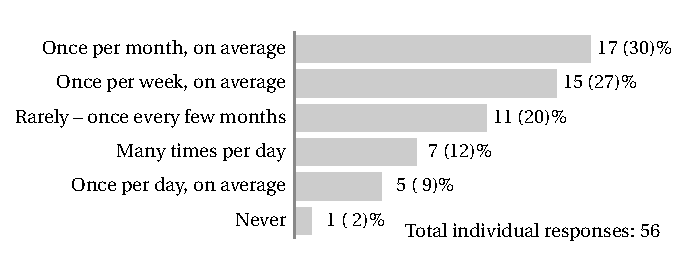
\includegraphics[width=3in]{files/plots/bar-graph-how-often-src.pdf}
  \caption{Responses to the question  ``How often do you search online for software source code?''  Predefined answer choices were presented as the mutually-exclusive multiple choices shown on the vertical axis.}
  \label{how-often-search-for-src}
\end{figure}

\clearpage

\subsection{RQ1: \rqonetext}
\label{results-rqone}

As mentioned above, after the demographics questions, the remaining questions in the survey questions were only shown if respondents indicated they had a choice in selecting the software they used.  All respondents indicated they have some choice in the software they use.

To assess how people located or discovered ready-to-run software, we asked ``When you need to find ready-to-run software for a particular task, how do you go about finding software?''  The question provided multiple nonexclusive answer choices together with a free-text ``Other'' option.  The predefined answer options were developed based on similar questions posed in other surveys~\citep{sim_2011, bajrachary_2009, linstead_2009} and the results of our pilot run.  Respondents were free to choose more than one answer.  Figure~\ref{how-find-ready-to-run} summarizes the results.  We separated the responses based on how individuals answered the yes/no question about being involved in software development (Figure~\ref{years}).  The graph is sorted by the sum of responses across developers and nondevelopers for each answer category.

\begin{figure}[bht]
  \centering
  \includefile{files/plots/how-find-ready-to-run-v4.pdf}
  \caption{Responses to the question ``When you need to find ready-to-run software for a particular task, how do you go about finding software?'' Answer choices were nonexclusive.  All \totalRespondents survey participants answered this question; results are subdivided according to respondents' answers to the question in Figure~\ref{years}, where \totalDevelopers people answered ``Yes'' to involvement in software development and 13 answered ``No''.  Percentages are calculated by subgroup.}
  \label{how-find-ready-to-run}
\end{figure}



\subsection{RQ2: \rqtwotext}
\label{results-rqtwo}

We sought to understand the selection and evaluation criteria that may come into play when users try to find ready-to-run software.  We posed the question ``In general, how important are the following characteristics when you are searching for ready-to-run software for a task?''  For the answer options, we provided a two-dimensional grid with different predefined criteria as the rows, and values on a unipolar rating scale for the columns.  The available values on the scale were ``Rarely or never important'', ``Somewhat or occasionally important'', ``Average importance'', ``Usually of above-average importance'', and ``Essential''. Figure~\ref{criteria-ready-to-run} summarizes the results.  To indicate which criteria respondents indicated they used, the rows of the graph are sorted by a percentage calculated as the sum of ``Essential'', ``Usually of above-average importance'' and ``Average importance'' ratings divided by the number of possible responses.  Not all participants chose to provide a value for every criterion.

% 2016-04-20 <mhucka@caltech.edu> I manually recalculated percentages based on the number of responses to the question (69), not the numbers per characteristic.  So for instance, for "availability of specific features", this resulted in (36 + 27)/69 = 91%.

\begin{figure}[t]
  \centering
  \includefile{files/plots/bar-graph-criteria-ready-to-run-reranked-v2.pdf}
  \caption{Responses to the question ``In general, how important are the following characteristics when you are searching for ready-to-run software for a task?'' All \totalRespondents respondents answered the question, but not all respondents chose to select an option for every possible characteristic.  Responses are ranked by a percentage calculated from the sum of the number of ``Essential'', ``Usually of above-average importance'' and ``Average importance'' ratings for each option divided by the total number of possible responses (\totalRespondents).}
  \label{criteria-ready-to-run}
\end{figure}

\clearpage

\subsection{RQ3: \rqthreetext}
\label{results-rqthree}

The currently-available catalogs of software are highly heterogeneous in their features and the information they present to users~\citep[e.g.,][]{nasa2016software, hempel2016xsede, darpa2015open, allen_2012, noy2009bioportal, hucka2016software, gleeson2016current, browne1995netlib, bonisch_2013}.  To help inform the development of improved catalogs, we sought to determine what kind of information users find important to provide about software.  We posed the following question of all participants who indicated they had the freedom to choose software (not only those who indicated they developed software): ``Suppose that it were possible to create a public, searchable catalog or index of software, one that would record information about software of all kinds found anywhere.  What kind of information would you find most useful to include for each entry in such a catalog or index?''  As with most other questions in our survey, we provided answer choices as nonexclusive multiple choices, with an additional free-text option titled ``Other''.  All \totalRespondents participants to our survey replied to this question.  Figure~\ref{info-to-include} summarizes the results.  We separated the responses based on how individuals answered the yes/no question about being involved in software development (Figure~\ref{years}).  The graph in Figure~\ref{info-to-include} is sorted by sum of responses across developers and nondevelopers for each answer category.

\begin{figure}[tbh]
  \centering
  \includefile{files/plots/info-to-include-in-index-v5.pdf}
  \caption{Answers to the question ``Suppose that it were possible to create a public, searchable catalog or index of software, one that would record information about software of all kinds found anywhere. What kind of information would you find most useful to include for each entry in such a catalog or index?'' There were 24 predefined items and a slot for free text under ``Other''.  Choices were nonexclusive.  All 69 survey respondents answered this question; results are shown subdivided according to participants' answers to the question in Figure~\ref{years} (left).  The graph is sorted by totals; e.g., ``Name of software'' was the third most selected choice across both developers and nondevelopers.}
  \label{info-to-include}
\end{figure}

\clearpage


\subsection{RQ4: \rqfourtext}
\label{results-rqfour}

As explained in Section~\ref{results-demographics}, the questions concerning searching for source code (RQ4, as well as RQ5 in the next section) were further gated by the question ``How often do you search online for software source code?''  A total of \totalSearchers participants indicated they searched for source code at least some of the time.  These participants were shown additional questions, including ``What are some approaches you have used to look for source code in the past?''.    Answer options were nonexclusive multiple choices, including an ``Other'' option with a field for free-text input.  Figure~\ref{how-find-src} provides a summary of the results.  This question was answered by all \totalSearchers participants who indicated that they searched for source code at least some of the time (Figure~\ref{how-often-search-for-src}).

\begin{figure}[thb]
  \centering
  \includefile{files/plots/how-find-src.pdf}
  \caption{Responses to the question ``What are some approaches you have used to look for source code in the past?''  This question offered the first eleven predefined categories and an additional slot for free text under ``Other''.  Answer choices were nonexclusive.  A total of \totalSearchers respondents answered this question.}
  \label{how-find-src}
\end{figure}


\subsection{RQ5: \rqfivetext}
\label{results-rqfive}

From our own experiences, we know a search for software can fail for a variety of reasons.  This motivated our inclusion of another question in the survey: ``What are some factors that have hindered your ability to FIND source code in the past?''  The question included a variety of nonexclusive predefined options, along with an ``Other'' option offering a free-text input field.  The results are summarized in Figure~\ref{factors-that-hindered}.

\begin{figure}[hbt]
  \centering
  \includefile{files/plots/factors-that-hindered-finding-src.pdf}
  \caption{Responses to the question ``What are some factors that have hindered your ability to FIND source code in the past?'' This question offered the first six predefined categories and an additional slot for free text under ``Other''.  Answer choices were nonexclusive.  A total of 52 survey respondents answered this question.}
  \label{factors-that-hindered}
\end{figure}

Six out of 52 respondents provided ``Other'' answers.  Three of these were simply explanatory but did not add to the categories listed, two participants cited lack of documentation as a hindrance to either locating or evaluating software, and the third hindrance noted by a respondent was ``Some scientific software is hidden from search engines as authors did not bother to put it online or make a small website for it.''

\clearpage


\section{Discussion}
\label{discussion}

In what follows, we discuss the results in the same order and with the same headings as they were presented in the previous section.

\subsection{Demographics}
\label{discussion-demographics}

Most of our survey respondents worked in three areas: physical sciences, computing and mathematical sciences, and biology and biological engineering (Figure~\ref{disciplines}). The responses to the remaining demographic questions (Section~\ref{results-demographics}) are consistent with prosaic expectations for the targeted scientific communities.  We expected to reach computer-literate individuals, and due to the distribution channels used, we most likely reached those working in research environments.  This is similar to other related studies such as that by \citet{lawrence2015science}.

Languages such as Python and Java are popular in these settings, and our survey's numbers for languages are consistent with those of a recent Stack~Overflow survey~\citep{stackexchange2016survey} for ``most popular technologies per dev type'' for their participants who chose ``Math \& Data''.  Most of our respondents indicated involvement in software development, and their typical team sizes were small, with 77\% being groups of~1 to~5 persons.  This is common in scientific software development, especially in academia, and more generally in open-source communities~\citep{sojer2010code}.  The fact that many respondents indicated they had multiple roles is also consistent---small teams generally require members to take on more than one role.

Among the 81\% of the total \totalRespondents respondents who were shown the section for software developers, the median number of years of experience was 20 (see Figure~\ref{years}). This suggests that the typical respondent is mid-career or part of the pre-mobile device generation.  Of these, 70\% (equal to 56\% of the overall \totalRespondents respondents) indicated that they were also primarily responsible for project management and/or software architecture, which are traditionally more senior roles.  The demographic data may thus indicate a bias in responses against more junior members of the respective communities, such as students and postdocs.  This is worth keeping in mind because junior members may have different search criteria and development experiences than more experienced colleagues. The possibility should be borne in mind when interpreting the survey results in the following sections. The cause of this distribution is unknown.


\subsection{RQ1: \rqonetext}
\label{discussion-rqone}

Figure~\ref{how-find-ready-to-run} summarizes the responses about how people find ready-to-run software.  For both software developers and nondevelopers, the top three choices were (a) using general search engines, (b) asking colleagues and (c) looking in the literature.  However, developers differed from nondevelopers in their frequency of selection of these choices: the top choice for developers (93\%) was search engines, whereas for nondevelopers, it was personal recommendations (92\%).  An even larger difference is evident in the use of social help sites such as Stack Overflow, with very few nondevelopers (15\%) indicating they used this approach.  A similar difference is exhibited with respect to searching public software project repositories such as SourceForge and GitHub, with nondevelopers far less likely to indicate they use that approach.  While it is perhaps not surprising that developers would be more familiar with these resources and thus recognizing them as viable options for finding software, the results demonstrate a difference in approaches used by developers versus nondevelopers.

General social media sites such as Facebook appear to be underutilized by both subsets of respondents when searching for ready-to-run software, although nondevelopers were nearly twice as likely to indicate they use these resources as a way to find software.  However, both subgroups rarely seem to use domain-specific catalogs.  This last result is surprising.  A possible explanation is that people may expect general search engines such as Google to index the domain-specific catalogs, and thus, that searching the former will subsume the latter.  This does happen in practice: results from at least some of the domain-specific catalogs can easily be demonstrated to show up in Google search outputs, though using the domain catalogs \emph{directly} will usually produce fewer, more relevant results.  A second possibility is it reflects a belief that such resources are too narrowly focused in scope for their needs.  A third possibility is that the results reflect ignorance of the existence of topical indexes.  Future research should probe this issue further and seek to understand the reasons behind this result.

Finally, the write-in answers for ``Other'' revealed a category of options we did not anticipate: the use of network-based software package installation systems such as the systems available for the different Linux operating system distributions.  In retrospect, this is an oversight in our list of predefined categories---the package management systems do offer some search capabilities, and thus, this is indeed another way for a person to find ready-to-run software.  Future surveys should include this as a predefined answer choice.


\subsection{RQ2: \rqtwotext}
\label{discussion-rqtwo}

The results of Figure~\ref{criteria-ready-to-run} indicate that the most important search criterion is the availability of specific features (96\%) in the software.  In fact, it was the only characteristic for which none of the respondents chose ``Somewhat or occasionally important'' or ``Rarely or never important''.  The high ranking of this characteristic is unsurprising: after all, if one is searching for software for a task, paying attention to the software's feature set is paramount.  The results also show that support for specific data standards and file formats (93\%) and software price (91\%) are also major considerations, which may reflect the culture of scientific computing.  Operating system requirements (88\%) scored highly, as did quality of documentation (86\%) and how easy the software is to learn (81\%).

How software is implemented in terms of programming language (42\%) and the particular software architecture (35\%) were deemed relatively unimportant.  We speculate that this may be simply because if one is looking for ready-to-run tools, the details of the implementation may not matter as much---it may be that other operational constraints, such as operating system support, may be more pressing constraints than how the software is written.

Quality and support aspects of the software appear to be secondary considerations as far as information to put in a software catalog.  Both the reputation of the developer (61\%) and the level of software support (59\%) were rated in the middle.  A possible explanation for this result is that once the software is installed, users in our sample expect that they can find their own solutions to any possible problems encountered, and that they are less concerned about future software updates. This may reflect the culture of software use in scientific computing; anecdotally, we find these users to be accustomed to less polished software and having lower expectations.  By contrast, in consumer or commercial environments, software is often closed-source, licenses are purchased with implied support, and updates are expected (and often issued automatically).

% A more surprising result is that other people's opinions of the software (22\%) and similarity to other software (12\%) did not rank higher.  It is possible that users resort to searching for software only when they lack other means of making selections, such as no word-of-mouth recommendations. In those cases, the approval rating of the software or its apparent familiarity may be largely ignored in favor of other criteria.  Future surveys or interviews could investigate these points more deeply.

% A surprising result is that, even though the question explicitly concerned ready-to-use software, the availability of the source code (62\%) and its licensing (55\%) were still relatively important considerations. This may reflect our particular population: a large fraction of responders identified themselves as developers. Such users are more likely to be capable and willing to alter the software to meet their specific requirements; thus, paying attention to source code and its licensing may be important for them.

We can compare these results to those of \citet{lawrence2015science} with respect to their question about important factors users consider when adopting new technology.  There are notable differences.  For example, in their survey, the highest-ranked factor was ``documentation available'', while in our survey, ``quality of documentation'' (the closest matching category) ranked sixth overall.  Their second-ranked factor, ``ability to adapt/customize'' is closed to our ``how easy the software is to extend'', which ranked seventeenth in our survey.  While it is true that our survey included many more possible criteria, and in addition, some criteria in Lawrence et al.'s survey question were coarser in detail, many items in both surveys are comparable, so these two differences alone are unlikely to explain the results.  We hypothesize two possibilities.  First, the context of their survey was scientific computing gateways, whereas our survey was not focused on this and considered people working with any kind of software environment.  This may influence the criteria people use to select between software options.  Second, it is possible that the rankings are influenced by the different answer formats: we asked participants to rank the importance of each criterion, while Lawrence et al.\ asked respondents pick their top three criteria.

Finally, it is interesting to compare these results with those of studies on desirable traits for successful open-source software projects~\citep[e.g.,][]{subramaniam2009determinants, lee2009measuring, crowston2003defining, crowston2006information, sen2012open, lee2009measuring}.  Intuitively, we expect the criteria should align: the features that people say they use to discriminate between choices when looking for software are presumably the same that differentiate successful software efforts from unsuccessful ones.  And in fact, it does turn out that code quality, documentation quality, price, and licensing terms are recognized indicators of success~\citep{subramaniam2009determinants, lee2009measuring, crowston2003defining, crowston2006information}; however, as mentioned above, our survey participants seemed to rate developers' reputations and other people's opinions of software as of middling importance, which does not align with studies about traits of successful software projects.


\subsection{RQ3: \rqthreetext}
\label{discussion-rqthree}

Figure~\ref{info-to-include} reports the results for the question ``Suppose that it were possible to create a public, searchable catalog or index of software, one that would record information about software of all kinds found anywhere.  What kind of information would you find most useful to include for each entry in such a catalog or index?''   When viewed across the subgroups of developers and nondevelopers, the five most-chosen characteristics to include were the operating system(s) supported, the purpose of the software, the name of the software, the domain of application, and license terms---all of which are very basic traits that are logically relevant to anyone looking for software.  Nondevelopers particularly favored the name and purpose as their two most-often chosen features to be included in a catalog.  (100\% of nondevelopers selected them.)  After these, the next most-often chosen were a URL for a home page, the data formats supported, and how recently the software was updated.

As might be expected, more developers than nondevelopers chose availability of source code as well as programming language as characteristics they want to see indexed.  In other respects, the trend for nondevelopers followed the same pattern as for developers, with one interesting exception: the availability of support or help was ranked by nondevelopers as highly as the home page URL.  By comparison, developers chose the availability of bug/issue trackers as often as they chose availability of support or help.  A possible explanation that in the minds of developers, support options and issue trackers may be more or less synonymous, whereas nondevelopers may be less inclined to use bug trackers and more inclined to simply contact the software's support address or personnel.

Details about the software, such as the types of user interfaces offered, a programmable API, and the programming language used to implement the software, were of middle importance to survey participants.  It came as a surprise, however, that more formal indicators of software development rigor---such as test cases, well-commented code, and metrics evaluating code quality---ranked relatively low, even for developers.  We expected developers to be more discerning about the quality of software they choose.  A possible explanation is that developers may simply assume they will need to take a closer personal look at any software they choose, so they don't regard it as important to include this information in a software index.  This is another aspect of the results that would be worth investigating more deeply in future work.

Finally, ten individuals wrote additional text in the ``Other'' field of the question.  Analysis of these responses revealed that one answer was similar enough to the predefined categories that we included it in the counts shown in the graph, and one response was not interpretable.  The remaining write-in values constituted sufficiently different categories of information that they were not truly subsumed by any of the options we provided.  The following are the distinct themes that were raised in these responses:

\begin{itemize}[itemsep=-0.5ex]

\item Price (two mentions)
\item Size of the user base (two mentions)
\item Availability of documentation (two mentions)
\item Size of the software
\item Whether it is packaged for Debian
\item URL of version control repository
\item List of plug-ins available
\item List of similar tools
\item Stability of parent organization

\end{itemize}


\subsection{RQ4: \rqfourtext}
\label{discussion-rqfour}

The responses to this question revealed that the use of general search engines was the most popular approach (91\%), followed by asking colleagues (53\%), and in third place, a tie between consulting the literature and searching in repositories such as SourceForge, GitHub and BitBucket (45\% each).  This is consistent with findings in some other published studies \citep[e.g.,][]{lawrence2015science}, though the relative percentages are different.

The use of specialized software indexes such as ASCL.net ranked much lower (24\%), as did searching code collections in one's organization (22\%).  Code search sites such as Open~Hub ranked even lower (18\%), and the use of social media systems such as Twitter, Facebook and LinkedIn ranked lower still (9\%).  Out of the four write-in ``Other'' answers, one was clearly in the same category as a predefined option, so we adjusted the counts accordingly; the other three were ``O'Reilly books'', ``Look at the web page for that software!'' and ``What libraries are used by other software that I like?''  These last three represent additional approaches not anticipated in our set of predefined answer choices.

These results show that close to half of respondents search project repositories such as GitHub when looking for source code, but unexpectedly, this approach is no more popular than looking in the scientific literature.  This may reflect a population sample bias towards researchers in our study: \emph{outside} of research environments, developers may be less likely look in the research literature as often as they search in GitHub.  On the other hand, we were surprised at the low ranking of searching topical software indexes.

How do these results compare to those of RQ1, which asked about finding ready-to-run software?  Although similar, the two questions were not identical: we offered three different answer choices because the contexts lent themselves to some different actions, and in addition, the question from Figure~\ref{how-find-ready-to-run} involved both developers and nondevelopers, whereas \emph{this} question involved \emph{only} developers.  Nevertheless, we can compare the common subset of answer categories and the subset of respondents in Figure~\ref{how-find-ready-to-run} who identified themselves as software developers.  We present the results in Figure~\ref{compare-how-find}.

\begin{figure}[bht]
  \centering
  \includefile{files/plots/compare-how-find-v2.pdf}
  \caption{Comparison of the results from \ref{how-find-ready-to-run} and \ref{how-find-src} for the overlapping answer categories. (Left) Subset of results from Figure~\ref{how-find-ready-to-run} for the \totalDevelopers respondents who indicated they were involved in software development.  The results have been expressed as percentages of the total number of responses for that subgroup of people.  (Right) Reproduction of the results of Figure~\ref{how-find-src}.}
  \label{compare-how-find}
\end{figure}

This shows that the top three approaches for finding \emph{both} ready-to-run software and source code are identical: searching the Web, asking colleagues, and looking in the literature.  When looking for source code, searching public repositories such as SourceForge and GitHub rises in popularity; while this is to be expected given the nature of the task and the fact that the respondents were software developers, the approach still only tied with searching the literature.

Some more unexpected results reveal themselves.  First, asking colleagues for opinions is far less common when searching for source code than when searching for ready-to-run software (53\% versus 80\%).  We have no hypothesis to explain this difference.  A second unexpected result is that the use of social help sites such as Stack Overflow was selected less frequently (36\%) when searching for source code than when searching for ready-to-run software (45\%).  Considering that Stack Overflow is one of the most popular online resources for software developers today, this result is counterintuitive.  Two possible explanations present themselves.  First, people may expect that using general-purpose search engines such as Google will return results from Stack Overflow and similar sites, and thus, they may simply not bother searching in the specialized sites directly.  A second possible explanation may come from considering responses to the question in the next section below, on the failure of past code searches: people cited an inability to find any code suitable for their purposes (69\%) and a belief that the requirements were too unique (63\%).  Perhaps these experiences and beliefs temper people's expectations of the potential for finding solutions through social help sites.  Future surveys should explore this question more deeply.

There is another surprising result: using software catalogs was more popular when the task was searching for source code compared to searching for ready-to-run software.  Indexes and catalogs do not offer \emph{source code search} per se, though source code may be available elsewhere (e.g., on the software's home page or repository).  Since developers cannot search inside source code from the catalogs, or in most cases even get a sense for the architecture of the software from the catalog descriptions alone, our intuition was that the indexes would be more useful for finding ready-to-run software---the opposite of what the survey revealed.  The reasons for this is another opportunity for future research.

Finally, we note that the use of software indexes was still quite low overall (12\% in the context of finding ready-to-run software, 22\% in the context of source code).  It ranked far lower than, for example, searching the literature, despite that software indexes are arguably much better suited to the task of finding software in a given domain or for a given purpose.  The same potential explanations we noted in Section~\ref{discussion-rqone} may apply here: namely, respondents may expect searching in Google will subsume searching in the specialized indexes, or participants may believe the indexes are too narrowly focused, or they may simply not be sufficiently aware of their existence.  More generally, this result indicates that the developers of software catalogs continue to face challenges in producing systems that users find sufficiently compelling.


\subsection{RQ5: \rqfivetext}
\label{discussion-rqfive}

The results of our question about search failures (Figure~\ref{factors-that-hindered}) show that the largest hindrance is simply finding a match to one's needs, either because of difficulty finding suitable working software or because none of the options found satisfy requirements.  Time limitations also often (46\%) impact the ability to conduct proper searches for source code or to evaluate the results.  This is may be due to the large number of results that general-purpose search engines can return, which in turn may make it difficult to find suitable results easily.  (After all, the ranking systems of general-purpose search engines such as Google are optimizing for a commercial metric, such as potential advertising revenue, rather than metrics more pertinent to searching for software.)

The results also suggest that software licensing (12\%) was a minor hindrance, even though it was a relatively important criterion for ready-to-use software (Section~\ref{results-rqtwo}).  This suggests that intellectual property information is not sufficiently visible during searches.  This is consistent with the format of results presented by Google and similar general-purpose search engines: they do not usually contain license information, unless it happens to be the in the first few words of the text fragment presented as part of a given search result.

Finally, one of the ``Other'' results written by respondents noted that some software packages lack web pages or other kinds of online presences.  This is a notable observation.  In effect, it means that the software is hidden from search engines, and may be hidden from search in social coding sites and social media as well.  Unfortunately, we do not have data about the types of software in this category.  Could it be that these ``hidden'' software packages are more likely to be older, non-commercial software? After all, commercial efforts are likely to seek to maximize publicity (in order to increase sales), while newer open-source efforts are likely to take advantage of online systems such as GitHub.  This is a question that could be probed in future surveys.

Overal, our results are very similar to those of \citet{samadi_2004}.  For our question about what factors hindered people from finding software (Section~\ref{results-rqfive}), the most popular reason was finding a match to one's needs.


\section{Conclusions}
\label{conclusions}

% When asked, many people say they look for software by searching the Web with a general-purpose search engine~\citep{samadi_2004, umarji_2008}.  Despite its popularity, this approach suffers from significant problems: Web searches can yield dozens of viable candidates---and millions of irrelevant results.  Moreover, some questions cannot be answered through Web searches without substantial additional effort, such as what are the \emph{specific} characteristics of each software tool or how do tools \emph{differ} from each other.  Many researchers also look in the scientific literature to learn what others have used for similar tasks~\citep{lawrence2015science, joppa2013troubling}.  Searching the literature can produce more relevant results and provide other information, but it suffers from limitations too: publications are static documents that may not reflect a tool's current capabilities~\citep{wren_2004}, and moreover, not all publications describe the software they use~\citep{howison2015software}.  Still other methods for finding software include asking colleagues, asking on social media, searching scientific computing gateways, and more.  None of these 

Before the advent of the World Wide Web, before even the advent of the current Internet, it was arguably easier to find software---there was less of it, and there were simply fewer places to look.  Initially, bulletin boards and archive sites using FTP made software available for copying by anonymous users over telephone networks; later, the Usenet culture~\citep{emerson1983usenet} of the 1980's encouraged widespread sharing and even devoted a newsgroup (\emph{comp.sources}) to the exchange of software source code.  Fast-forward to today, and the staggering wealth of software resources available to users is both a blessing and a curse: one can simultaneously feel that for any given task, ``surely someone has already written software to do this,'' and yet an attempt to find suitable software can seem like falling into a rabbit hole.

\subsection{How people find software today}

So what \emph{do} users do today when they want to find software?  This survey was an attempt to gain insight into the approaches used by people working in science and engineering, as well as the criteria that they apply to select between alternative software choices.  Our participants worked primarily in the physical, computing, mathematical and biological sciences; the majority were involved in software development and had a mean of 20 years of experience; most worked in small groups; and all had some degree of choice in the software they used.  The majority spent over 50\% of their day using software; this is somewhat higher than some other studies have reported  \citep[e.g.,][found scientists spent 40\% of their time using scientific software]{hannay_2009}.

The survey results help identify a number of current community practices in searching for both ready-to-use software and source code:

\begin{enumerate}

\item When searching for ready-to-run software (RQ1), the top three approaches overall were are: (i) search the Web with general-purpose search engines, (ii) ask colleagues, (iii) look in the scientific literature.  After these top three, the next most commonly stated approaches differed between those respondents who self-identified as being involved in software development and those did not: more developers indicated asking on social help sites such as Stack Overflow and searching in public software repositories such as GitHub (in that order), while non-developers indicated following their organization's guidelines and a tie between asking on public mailing lists and asking on social media.

\item The top five criteria given above-average weight when searching for ready-to-run software are: (i) availability of specific features, (ii) support for specific data standards and file formats, (iii) price, (iv) apparent quality of the software, and (v) operating system requirements.

\item Regarding information people would like to see in a catalog or index of ready-to-run software, a total of 15 features were indicated as having above-average value by at least 50\% of the respondents; of these characteristics, the operating system supported, purpose of software, name of software, domain/field of application, and licensing terms were the five most-often requested features.  Developers displayed slightly different preferences compared with nondevelopers, notably with respect to the availability of support or help for a given software product, but on the whole, both subgroups displayed similar preferences.

\item The top five approaches used by developers in science and engineering to search for source code are almost identical to those they use to find ready-to-run software.  They are: (i) search the Web with general-purpose search engines, (ii) ask colleagues, (iii) look in the scientific literature, (iv) search in public software project repository sites such as GitHub, and (v) look in social help sites such as Stack Overflow.  % Somewhat surprisingly, developers were more likely to search programming-oriented sites such as Stack Overflow when looking for \emph{ready-to-run} software than when looking for source code.

\item The top three reasons developers are sometimes \emph{unable} to find source code are: (i) unable to locate suitable software, (ii) requirements are too unique, and (iii) insufficient time to search or evaluate options.  Concerns about intellectual property issues ranked low.

\end{enumerate}

The results above have implications for the development of better resources for locating software.  In common with other surveys, we found that more people indicate they use general Web search engines than any other approach for finding both ready-to-run software and source code.  This implies that for any specialized resource such as a software catalog to gain popularity, it must be indexed by Google and other search engines so that users can find its content via general Web searches.  In addition, the five attributes most important to our respondents when they are seeking software are (i) specific features, (ii) specific data standards supported, (iii) price, (iv) operating system requirements, and (v) apparent quality.  This implies that improving people's ability to obtain this information would improve their ability to find software in different situations.  Finally, software cataloging efforts would benefit by focusing on the most desirable information items revealed by our survey (Figure~\ref{info-to-include}).

% These have implications for development of catalogs or other resources to help people find software.  

\subsection{Lessons for future surveys}

Analyzing the survey results has led us to recognize aspects of the survey that could have been improved.  First, in the demographic profile questions (Section~\ref{results-demographics}), it would have been useful to gather more specific data.  For example, the work fields question could have offered finer-grained options, and additional questions could have asked participants about their institutional affiliation (e.g., educational, government, industry) as well as their work roles (e.g., student, staff, faculty).  Of course, the benefits of additional questions must be weighed against respondents' patience for filling out long surveys.

Second, the questions asking about software search could have had an explicit answer choice about the use of scientific gateways.  The survey questions generally did not mention gateways or portals explicitly; the closest was the question discussed in Figure~\ref{info-to-include}, which included workflow environments as an answer choice.  Based on the responses reported in Figure~\ref{info-to-include}, one quarter of the respondents consider support for workflow environments a criterion in selecting software.  Since we did not ask about it explicitly, it is unclear whether any of the participants had the use of gateways in mind and framed their responses accordingly.  It is also not clear what effect this would have had on their responses.  Gateways concentrate software resources in one location and typically provide an index or other means of finding software provided by the gateway, and it is conceivable that this may change the nature of how users think of finding software or the criteria they use to discriminate between available alternatives.  It is therefore possible that this is a confounding factor in our results.  Future surveys should address this aspect explicitly.

Third, future work must strive to increase the response rate.  While we believe the present survey's results are accurate for the sample of people who finished the survey, we must also acknowledge that a response rate of \populationResponseRate is disappointing.  It is widely asserted that Web-based surveys often encounter low rates~\cite[e.g.,][]{kitchenham_2008, couper2000review, couper2008web}; in our experience, many studies even fail to disclose the response rate, or claim a rate without reporting the number of potential recipients, leaving in question the accuracy of the rate.  However, of the published surveys that disclose both the number of potential recipients and the number of completed responses received~\cite[e.g.,][]{wu2007empirical, bauer2014exploratory, kalliamvakou_2014, lawrence2015science, sojer2010reusing}, the values often have been higher.  For example, \citet{sojer2010reusing} reported 9.7\% and \citet{lawrence2015science} obtained 17\%, albeit with a highly motivated population.  One possible cause for our lower response rate may be the venues where we advertised the survey.  Our primary venues for soliciting participation were certain mailing lists and Facebook groups.  With respect to the mailing lists, some recipients may not have received the survey messages because automatic spam filters may have blocked the messages from their electronic mail inboxes.  This would mean that fewer people saw the invitations than the number of people subscribed to the mailing lists, artificially reducing the apparent response rate.  With respect to Facebook, some users may be have signed up long ago but they may rarely or never check the group we targeted.  The latter is especially plausible when we consider two other results of our survey: as shown in Figure~\ref{years}, respondents had a mean of 20 years of experience, and in Figure~\ref{compare-how-find}, social media of Twitter/Facebook/LinkedIn variety were little-used by participants for finding software.  If that reflects the overall population we reached and their broader pattern of social media use, then they may simply be of a generation that spends less time on Facebook than a younger generation of researchers.  Again, this would cause our estimated number of recipients to be higher than the actual number of people who saw the announcements in that venue.  Finally, it is possible that our announcements and/or the front page of the survey were simply not sufficiently motivational.


\section{Acknowledgments}

We thank
Alice Allen,
Daniel S. Katz,
Sarah M. Keating,
Matthias K\"{o}nig,
Allyson Lister,
Rajiv Ramnath,
Renee M. Rottner,
Lucian P. Smith, and
Linda J. Taddeo
for many comments and feedback on previous versions of this manuscript.
This work was supported by the USA National Science Foundation (award \#1533792).


\bibliographystyle{elsarticle-harv}
\bibliography{casics-survey.bib}

\end{document}
